\documentclass{article}
\usepackage{graphicx} % Required for inserting images
\usepackage[ngerman]{babel}
\usepackage{enumitem}
\usepackage{float}
\usepackage{chngcntr}
\usepackage{glossaries}
\usepackage{tabularx}
\counterwithin{figure}{section}
\counterwithin{table}{section}
\setlength\parindent{0pt}

\makeglossaries

\newglossaryentry{Attributsableitung}
{
    name=Attributsableitung,
    description={Platzhalter-Implementierung eines Glossar-Eintrags}
}

\newglossaryentry{Verkehrsmodell}
{
    name=Verkehrsmodell,
    description={Platzhalter-Implementierung eines Glossar-Eintrags}
}

\newglossaryentry{Discrete Choice}
{
    name=Discrete Choice,
    description={Platzhalter-Implementierung eines Glossar-Eintrags}
}

\newglossaryentry{Projektdatei}
{
    name=Projektdatei,
    description={Kann eine CSV-Datei, Attributsableitungen, Alternativen und Nutzenfunktionen beinhalten}
}

\newacronym{WK}{WK}{Wunschkriterium}

\newacronym{CSV}{CSV}{Comma-separated values}

\newglossaryentry{Alternative}
{
    name=Alternative,
    description={Ein alternatives Verkehrsmittel}
}

\title{PflichtenheftA \\ \large Einflussfaktoren auf die Verkehrsmittelwahl\\ -- Baukasten für Discrete Choice Modelle}
\author{Kevin Boehnke \\ \texttt{uxpkw@student.kit.edu}
\and Floriane Bresser \\ \texttt{uspvq@student.kit.edu}
\and Damian Reich \\ \texttt{uqppn@student.kit.edu}
\and Alissa Saleh \\ \texttt{unmbc@student.kit.edu}
\and Michael Schur \\ \texttt{ufkmz@student.kit.edu}}
\date{24. Mai 2023}

\begin{document}
\clearpage\maketitle\thispagestyle{empty}
\newpage
\clearpage\tableofcontents\thispagestyle{empty}
\newpage
\pagenumbering{arabic}

\section{Einleitung}

Im Alltag existieren viele Einflussfaktoren auf die Verkehrsmittelwahl, wie die demographische Entwicklung, Infrastrukturmaßnahmen, Veränderungen in Siedlungsstrukturen, Steuerungsmaßnahmen, veränderte Energiepreise oder Maßnahmen des Mobility Pricings. Zur Schaffung einer quantitativen Basis, die verkehrsplanerische, betriebswirtschaftliche und politische Entscheidungen unterstützt, werden Verkehrsmodelle eingesetzt.\newline

Ein Verkehrsnachfragemodell ist die Diskrete Entscheidungsmodellierung. In diesem werden jeder Wahlmöglichkeit Aufteilungs- und Nutzenfunktionen zugewiesen, die auf Parametern beruhen. Die Parameter werden mittels der Maximum-Likelihood-Schätzung aus Umfrageergebnissen geschätzt, in denen die Befragten Aussagen über ihr Verhalten bei der Verkehrsmittelwahl machen. Ebenfalls können Parameter mittels der Stated Choice Methode geschätzt werden. Diese basiert auf hypothetischen Entscheidungssituationen zwischen Alternativen mit zugewiesenen Attributen. Eine Stated Choice Parameterschätzung beginnt mit Entscheidungen über die Alternativen und ihrer Attribute und der Erwartung möglicher Nutzenfunktionen zur Optimierung des Designs des Stated Choice Experiment. Anschließend wird das Design implementiert und die Befragung umgesetzt. Im letzten Schritt soll das Aufbereiten der Daten und Abschätzen der Parameter erfolgen.\newline

Der Baukasten übernimmt dabei das Einlesen und Aufbereiten der Daten und ermöglicht durch Berechnungen im Rahmen der Modelle eine Schätzung und Visualisierung der Parameter. Durch die Möglichkeit individuell definierter Funktionen soll das Produkt diesen Ablauf vereinfachen und eine automatisierte Parameterschätzung sowie die Visualisierung der Modelle ermöglichen. 

\subsection{Anmerkungen}
Wunschkriterien außerhalb des Blocks \textbf{2 Zielbestimmung} werden durch (\textit{WK}) markiert.

\newpage
\section{Zielbestimmung}
Das Produkt unterstützt die Verkehrsingenieure dabei, Discrete Choice Modelle in der Verkehrsmittelwahl zu erstellen, modifizieren und visualisieren.
\subsection{Musskriterien}
\begin{itemize}
    \item[\textbf{/MK1/}] Der Nutzer kann Erhebungsdaten im CSV-Format importieren.
    \item[\textbf{/MK2/}] Der Nutzer kann Attributsableitungen hinzufügen, ändern, und löschen.
    \subitem Folgende Möglichkeiten stehen dem Nutzer zur Verfügung:
    \begin{itemize}[leftmargin=.7in]
        \item[\textbf{/MK2.1/}] Intervalle
        \item[\textbf{/MK2.2/}] Gruppen
        \item[\textbf{/MK2.3/}] Logische Ausdrücke
        \item[\textbf{/MK2.4/}] Vergleiche
    \end{itemize}
    \item[\textbf{/MK3/}] Der Nutzer kann Alternativen hinzufügen und löschen.
    \item[\textbf{/MK4/}] Der Nutzer kann für jede Alternative eine Nutzenfunktion definieren und ändern.
    \begin{itemize}[leftmargin=.7in]
        \item[\textbf{/MK4.1/}] Der Nutzer kann Linearkombinationen für die Nutzenfunktion verwenden.
    \end{itemize}
    \item[\textbf{/MK5/}] Der Nutzer kann die Parameter und Signifikanz aus gegebener Eingabe und Modellstruktur berechnen lassen.
    \item[\textbf{/MK6/}] Das Programm bietet eine Schnittstelle für andere Bibliotheken zur Parameterschätzung und Signifikanzgewinnung. 
    \begin{itemize}
        \item Es wird standardmäßig das Python Paket \textit{Biogeme} verwendet.
    \end{itemize}
    \item[\textbf{/MK7/}] Das Programm visualisiert die gewonnenen Parameter und Signifikanzniveaus.
    \item[\textbf{/MK8/}] Der Nutzer kann die Ergebnisse der Berechnung und die Visualisierung exportieren.
    \item[\textbf{/MK9/}] Der Nutzer kann die Tabelle im CSV-Format mit den Attributsableitungen exportieren.
    \item[\textbf{/MK10/}] Das Programm bietet eine Schnittstelle um die Parameteraufteilung zu erweitern oder einzuteilen anhand der Signifikanzniveaus.
    \item[\textbf{/MK11/}] Der Nutzer kann ein Projekt als Projektdatei speichern und laden.
\end{itemize}

\subsection{Wunschkriterien}
\begin{itemize}
    \item[\textbf{/WK1/}] Das Programm unterstützt arbiträre Funktionen für Attributsableitungen.
    \item[\textbf{/WK2/}] Der Nutzer kann die importierte CSV-Datei graphisch darstellen lassen.
    \item[\textbf{/WK3/}] Der Nutzer wird bei der Programmführung durch folgende Funktionen von der Software unterstützt:
    \begin{itemize}[leftmargin=.7in]
        \item[\textbf{/WK3.1/}] Autovervollständigung
        \item[\textbf{/WK3.2/}] Typhinweise
        \item[\textbf{/WK3.3/}] Fehlerunterbindung
    \end{itemize}
    \item[\textbf{/WK4/}] Die Nutzenfunktionen können wie folgt verschachtelt werden:
    \begin{itemize}[leftmargin=.7in]
        \item[\textbf{/WK4.1/}] Arithmetik: $\beta \cdot (T + (\beta_2 \cdot X_2 \cdots))$
        \item[\textbf{/WK4.2/}] Exponentialfunktionen: $\log(T)$, ${\rm e}^T$
        \item[\textbf{/WK4.3/}] Potenzen: $\beta \cdot X^3$
    \end{itemize}
    \item[\textbf{/WK5/}] Das Programm kann um andere Modell-Strukturen erweitert werden.
    \begin{itemize}
        \item Beispielsweise um das \textit{Nested Logit Model}
    \end{itemize}
    \item[\textbf{/WK6/}] Der Nutzer kann die Schwellwerte für die Signifikanz in der Visualisierung konfigurieren.
    \begin{itemize}
        \item Beispielsweise im \textit{Apollo Package}: $|T-Ratio | > 1.95$, $|Robust T-Ratio | > 1.95$
    \end{itemize}    
    \item[\textbf{/WK7/}] Das Programm bietet einen vollwertigen Algorithmus zur Bestimmung von Signifikanzgruppen und Aufteilungen.
    %\item[\textbf{/WK8/}] Die Anwendung kann auf einer Workstation, Windows Server, 8 Kerne (16 logische Kerne) ausgeführt werden. 
    
\end{itemize}
\subsection{Abgrenzungskriterien}

\newpage
\section{Produkteinsatz}
\subsection{Anwendungsbereiche}
Der vorgesehene Anwendungsbereich ist die Verkehrsmodellierung aus Befragungsdaten im Bereich der Verkehrswissenschaften. Die Anwendung eignet sich zur Modellierung für eine Prognose als Basis für verkehrsplanerische, betriebswirtschaftliche und politische Entscheidungen. Ebenso kann sie Verwendung in der Recherche finden.

\subsection{Zielgruppen}
Das Produkt richtet sich an Verkehrsingenieure und Verkehrswissenschaftler. Zur Verwendung sind keine Vorkenntnisse im Bereich Informatik notwendig. Ebenfalls wird eine Open Source Veröffentlichung angestrebt.
  
\subsection{Betriebsbedingungen}
Der Baukasten wird als Desktopanwendung konzipiert, die in Büroumgebung ausgeführt wird. Übliche Betriebsbedingungen sind die Nutzung zu konventionellen Arbeitszeiten. Es ist keine Beobachtung während der Ausführung notwendig, unbeaufsichtigter Betrieb wird unterstützt und die Ausführung kann unterbrochen und zu späteren Zeitpunkten fortgeführt werden. Zur Ausführung der Anwendung wird keine Internetverbindung benötigt.
Mindestanforderungen für den Baukasten ist ein Laptop mit 8 GB RAM, i5 (4 Kerne, 8 logische Kerne) und Betriebssystem Windows 10 oder Windows 11. Ebenfalls soll die Anwendung auf der Workstation mit Windows Server, 8 Kerne (16 logische Kerne) ausgeführt werden können (\textit{WK}).
\newpage

\section{Produktumgebung}
\subsection{Software}
\begin{itemize}
    \item Die Software wird in Python geschrieben.
    \item Betriebssystem: Windows 10 oder Windows 11
    \item Die Software wird als Open Source veröffentlicht und erweiterbar sein.
\end{itemize}
\subsection{Hardware}
\begin{itemize}
    \item Das Produkt ist eine Desktopanwendung.
    \begin{itemize}
        \item Mindestanforderung: Laptop, 8 GB RAM, Intel Core i5 (4 Kerne, 8 logische Kerne)
        \item (\textit{WK})\textit{: Workstation, Windows Server, 8 Kerne (16 logische Kerne)}
    \end{itemize}
\end{itemize}
\subsection{Schnittstelle}
\begin{itemize}
    \item Die Software nimmt Dateien im CSV-Format entgegen.
    \item Die Anwendung soll über eine Schnittstelle andere Bibliotheken zur Parameterschätzung einbinden können.
    \begin{itemize}
        \item beispielsweise das \textit{Apollo Package}
    \end{itemize}
\end{itemize}
\newpage

\section{Produktfunktionen}
\subsection{Funktionsübersicht}
Im Folgenden ist eine Übersicht der Produktfunktionen.
\begin{figure}[H]%
  \centering
  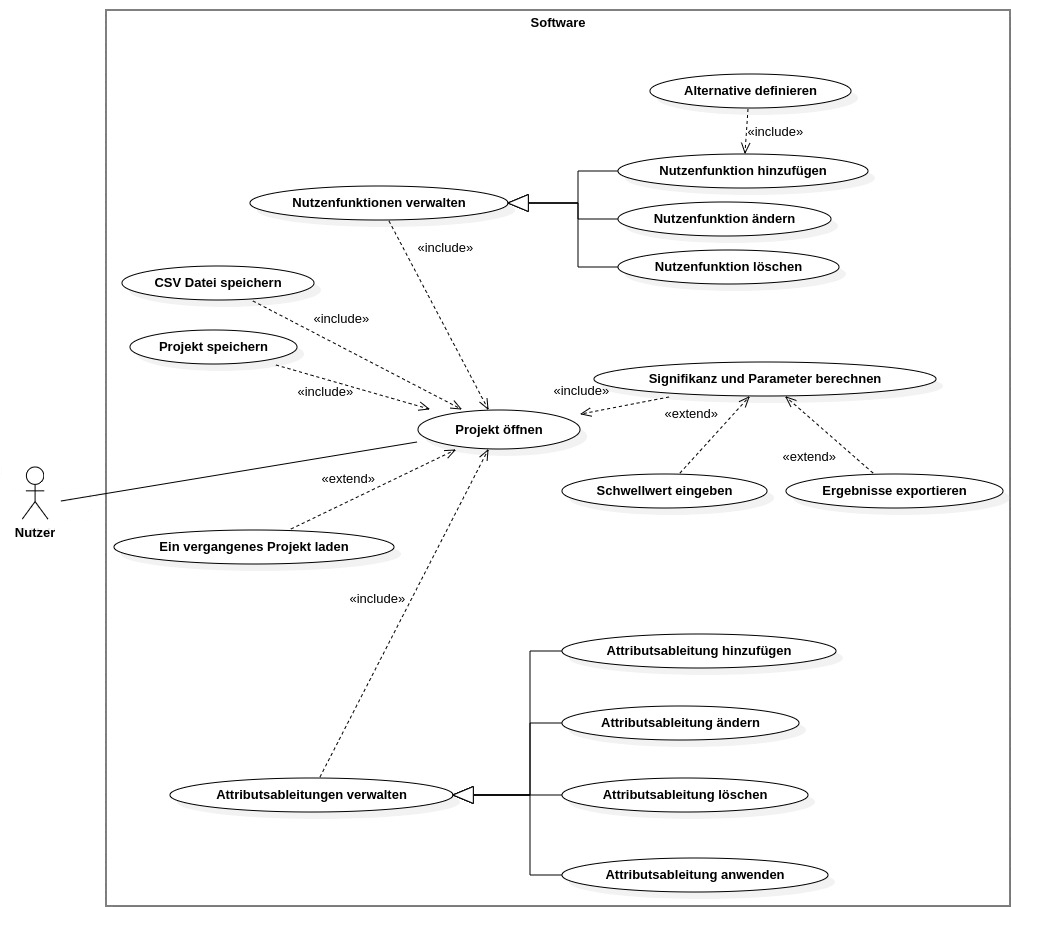
\includegraphics[width=15cm]{use case5.jpg}
  \caption{Use Case Diagramm}
\end{figure} 
\newpage
\textbf{/F10/} Projekt öffnen \\
\textbf{/F11/} Ein existierendes Projekt laden \\
\textbf{/F12/} Projekt speichern \\
\textbf{/F13/} CSV Datei speichern \\
\textbf{/F15/} Attributsableitungen hinzufügen \\
\textbf{/F16/} Attributsableitungen ändern \\
\textbf{/F17/} Attributsableitungen löschen \\
\textbf{/F18/} Attributsableitungen anwenden \\
\textbf{/F20/} Nutzenfunktionen eingeben \\
\textbf{/F21/} Nutzenfunktionen ändern \\
\textbf {/F22/} Nutzenfunktionen löschen \\
\textbf{/F25/} Signifikanzgenerierung \\
\textbf{/F28/} Ergebnisse exportieren \\
\textbf{/F30/} Schwellwerte konfigurieren
%\newpage
\\[0.5in]
\subsubsection*{/F10/ Projekt öffnen}
\underline {Ziel}:  Ein neues Projekt öffnen, in dem eine bereits existiernde CSV Datei geladen wird, welche die nötigen Erhebungsdaten beinhaltet. \\
\underline{Vorbedingung}: keine\\
\underline{Beschreibung}: Nutzer wählt die CSV Datei, welche im Laufe des Projekts bearbeitet wird.
\underline{Erfüllende Kriterien}: /MK1/; /WK2/
\subsubsection*{/F11/ Ein existierendes Projekt laden}
\underline{Ziel}: Auf einem bereits existierendes Projekt zugreifen. \\
\underline{Vorbedingung}: keine \\
\underline{Beschreibung}: statt ein neues Projekt zu starten, der Nutzer wählt die Projektdatei und lädt ihn.
\underline{Erfüllende Kriterien}: /MK1/;/MK10/;/WK2/
\subsubsection*{/F12/ Projekt speichern}
\underline{Ziel}: Bereits eingegebene Attributsableitungen, Nutzenfunktionen, Ergebnisse aus schon durchgeführten Berechnungen und Änderungen an dem CSV Datei speichern\\
\underline{Vorbedingung}: Projekt muss geöffnet sein \\
\underline{Beschreibung}: Der Nutzer klickt auf die Option Projekt speichern. \\
\underline{Erfüllende Kriterien}: /MK10/
\newpage
\subsubsection*{/F13/ CSV Datei speichern}
\underline{Ziel}: Die neue Tabelle (ursprüngliche Tabelle mit neuen Spalten) in einer neuen CSV Datei speichern\\
\underline{Vorbedingung}: Projekt muss geöffnet sein. \\
\underline{Beschreibung}: Nutzer klickt auf die Option CSV speichern.\\
\underline{Erfüllende Kriterien}: ??
\subsubsection*{/F15/ Attributsableitungen hinzufügen}
\underline{Ziel}: Neue Attributsableitungen definieren. \\
\underline{Vorbedingung}: Projekt muss geöffnet sein. \\
\underline{Beschreibung}: Nutzer gibt Funktion an. Wenn die Eingabe syntaktisch korrekt ist, wird sie hinzugefügt.\\
\underline{Erfüllende Kriterien}: /MK2/; /WK1/; /WK3/
\subsubsection*{/F16/ Attributsableitungen ändern}
\underline{Ziel}: Bereits existierende Attributsableitungen ändern. \\
\underline{Vorbedingung}: Projekt muss geöffnet sein. Existenz der Funktion, die geändert werden soll  \\
\underline{Beschreibung}: Die Funktion wird geändert, wenn die neue Eingabe syntaktisch korrekt ist.\\
\underline{Erfüllende Kriterien}:/MK2/; /WK1/; /WK3/
\subsubsection*{/F17/ Attributsableitungen löschen}
\underline{Ziel}: Erfolgreiche Löschung einer Attributsableitung. \\
\underline{Vorbedingung}: Projekt muss geöffnet sein. Existenz der Funktion, die gelöscht werden soll.\\
\underline{Beschreibung}: Nutzer löscht die Funktion. Sind durch die Funktion Spalten in der CSV Datei entstanden, so werden diese auch gelöscht. \\
\underline{Erfüllende Kriterien}: /MK2/
\subsubsection*{/F18/ Attributsableitungen anwenden}
\underline{Ziel}: Eingegebene Attributsableitungen anwenden. \\
\underline{Vorbedingung}: Attributsableitungen müssen vorher existieren; CSV Datei muss geöffnet sein. \\
\underline{Beschreibung}: Nutzer wählt die Ableitungen, die berechnet werden sollen. Durch die Anwendung werden neue Spalten in der CSV Datei entstehen.\\
\underline{Erfüllende Kriterien}: ??
\newpage
\subsubsection*{/F20/ Nutzenfunktionen einfügen}
\underline{Ziel}: Nutzenfunktionen definieren. \\
\underline{Vorbedingung}: Projekt muss geöffnet sein; Benötigte Spalten/Ableitungen müssen vorhanden sein.\\
\underline{Beschreibung}: Nutzer gibt die Nutzenfunktion ein. Sie soll eine Linearkombination sein. Wenn die eingegebene Nutzenfunktion korrekt ist (Linearkombination und benötigte Spalten existieren), wird sie hinzugefügt. Außerdem muss die Alternative dazu definiert werden. \\
\underline{Erfüllende Kriterien}: /MK3/; /MK4/; /WK4/
\subsubsection*{/F21/ Nutzenfunktionen ändern}
\underline{Ziel}: Nutzenfunktionen ändern.\\
\underline{Vorbedingung}: Projekt muss geöffnet sein; Die zu ändernde Nutzenfunktion muss existieren bzw. vorher eingegeben werden; Falls neue Spalten benutzt werden, müssen diese auch existieren \\
\underline{Beschreibung}: Nutzer ändert die bereits existierende Nutzenfunktion. Wenn die Änderungen korrekt sind werden sie umgesetzt. \\
\underline{Erfüllende Kriterien}: /MK4/; /WK4/
\subsubsection*{/F22/ Nutzenfunktionen löschen}
\underline{Ziel}: Nutzenfunktionen löschen.\\
\underline{Vorbedingung}: Projekt muss geöffnet sein; Die zu löschende Nutzenfunktion muss existieren. \\
\underline{Beschreibung}: Nutzer löscht die Nutzenfunktion. \\
\underline{Erfüllende Kriterien}: /MK3/;/MK4/
\subsubsection*{/F25/ Signifikanzgenerierung}
\underline{Ziel}: Signifikanz und die Parameter bestimmen. \\
\underline{Vorbedingung}: Projekt muss geöffnet sein; Nutzenfunktionen müssen schon definiert sein. \\
\underline{Beschreibung}: Nutzer gibt die Anweisung, Signifikanz zu bestimmen. Diese erfolgt automatisch mit Bestimmung der Parameter durch ( R Bibliothek Apollo oder Python Biogeme)?. Nach der Berechnung werden die Ergebnisse dem Nutzer gezeigt. \\
\underline{Erfüllende Kriterien}:/MK5/; /MK6/; /MK7/ 
\newpage
\subsubsection*{/F28/ Ergebnisse exportieren}
\underline{Ziel}: Ergebnisse der Signifikanz und  Parameter Berechnung exportieren \\
\underline{Vorbedingungen}: Projekt muss geöffnet sein; Signifikanz muss vorher berechnet werden. \\
\underline{Beschreibung}: Parameterwerte und Signifikanz werden in einer CSV Datei exportiert. \\
\underline{Erfüllende Kriterien}: /MK8/
\subsubsection*{/F30/ Schwellwerte konfigurieren}
\underline{Ziel}: Schwellwert ändern; Bestimmt welche Parameter hervorgehoben werden. \\
\underline{Vorbedingungen}: Projekt muss geöffnet sein; Berechnung der Signifikanz muss vorher erfolgt sein. \\
\underline{Beschreibung}: Nutzer ändert den Schwellwert.\\
\underline{Erfüllende Kriterien}: /WK6/

\clearpage
\section{Produktdaten}
Die Speicherung der Daten erfolgt ausschließlich lokal.
\subsection{Projektdaten}
Bei der Speicherung eines Projekts werden die folgenden Daten gespeichert. Für den Nutzer zugänglich werden D20, D30, D40 und D70 in einem Projektordner gespeichert.
\subsubsection*{/D10/ Rohdaten}
Die CSV Datei, die dem Projekt zugrunde liegt, wird unverändert gespeichert.
\subsubsection*{/D20/ Ableitungen}
Die benutzerdefinierten Ableitungen des Projektes werden separat als CSV Datei gespeichert.
\subsubsection*{/D30/ Signifikanzen}
Im Projekt errechnete Signifikanzen werden als separate CSV Datei gespeichert.
\subsubsection*{/D40/ Parameter}
Die berechneten Parameter werden als separate CSV Datei gespeichert.
\subsubsection*{/D50/ Verwendete Funktionen}
Die im Projekt verwendeten Funktionen werden projektabhängig als .json  Datei gespeichert. Die Speicherung erfolgt regelmäßig im Hintergrund.
\subsubsection*{/D60/ Ableitungsfunktion}
Benutzerdefinierte Ableitungsfunktionen werden projektabhängig als .json Datei gespeichert.
\subsubsection*{/D70/ CSV Datei mit Berechnungen}
Die vollständige CSV Datei, die sowohl Rohdaten als auch Attribute enthält wird temporär gespeichert.
\subsection{Nutzenfunktionen}
Die Speicherung der Nutzenfunktionen ist separat zu den Projekten und wird dem Nutzer nicht zur Verfügung gestellt.
\subsubsection*{/D80/ Nutzenfunktion}
Die benutzerdefinierten Nutzenfunktionen werden als separate Datei projektunabhängig gespeichert. Auf die gespeicherten Nutzenfunktionen kann von jedem Projekt aus zugegriffen werden.


\clearpage
\section{Produktleistungen}
\subsection{Bedienbarkeit}
\begin{itemize}
    \item[\textbf{/LB1/}] Die Berechnung der Ergebnisse kann jederzeit abgebrochen werden.
\end{itemize}
\subsection{Kommunikation}
\begin{itemize}
    \item[\textbf{/LK1/}] Das Laden einer korrupten CSV- oder Projektdatei wird mit einer Fehlermeldung abgebrochen. Das Programm wird dadurch nicht beeinträchtigt.
    \item[\textbf{/LK2/}] Ungültige Nutzenfunktionen werden visuell und mit Fehlermeldung markiert.
    \item[\textbf{/LK3/}] Ungültige Attributsableitungen werden visuell und mit Fehlermeldung markiert.
    \item[\textbf{/LK4/}] Das Laden einer Projektdatei mit ungültigen Nutzenfunktionen oder ungültigen Attributsableitungen wird dem Nutzer mit einer Fehlermeldung angemerkt. Die Projektdatei kann danach in das Programm geladen.
    \item[\textbf{/LK5/}] Werden durch das Laden einer CSV-Datei Nutzenfunktionen oder Attributsableitungen ungültig, wird der Nutzer davor gewarnt. Das Laden kann daraufhin abgebrochen oder durchgeführt werden.
\end{itemize}
\subsection{Performance}
\begin{itemize}
    \item[\textbf{/LP1/}] Das Importieren einer CSV-Datei ($\leq$ 500MB) erfolgt innerhalb von maximal 5 Sekunden.
    \item[\textbf{/LP2/}] Das Laden einer Projektdatei ($\leq$ 500MB CSV-Datei, $\leq$ 20 Alternativen, $\leq$ 30 Attributsableitungen) erfolgt innerhalb von maximal 10 Sekunden.
    \item[\textbf{/LP3/}] Die Berechnung der Ergebnisse und die Visualisierung erfolgt innerhalb von maximal 10 Sekunden.
    \item[\textbf{/LP4/}] Das Exportieren der Ergebnisse und der Visualisierung erfolgt innerhalb von maximal 5 Sekunden.
    \item[\textbf{/LP5/}] Das Exportieren der CSV-Datei mit den Attributsableitungen erfolgt innerhalb von maximal 3 Sekunden.
\end{itemize}

\clearpage
\section{Benutzerschnittstelle}
\begin{figure}[H]%
  \centering
  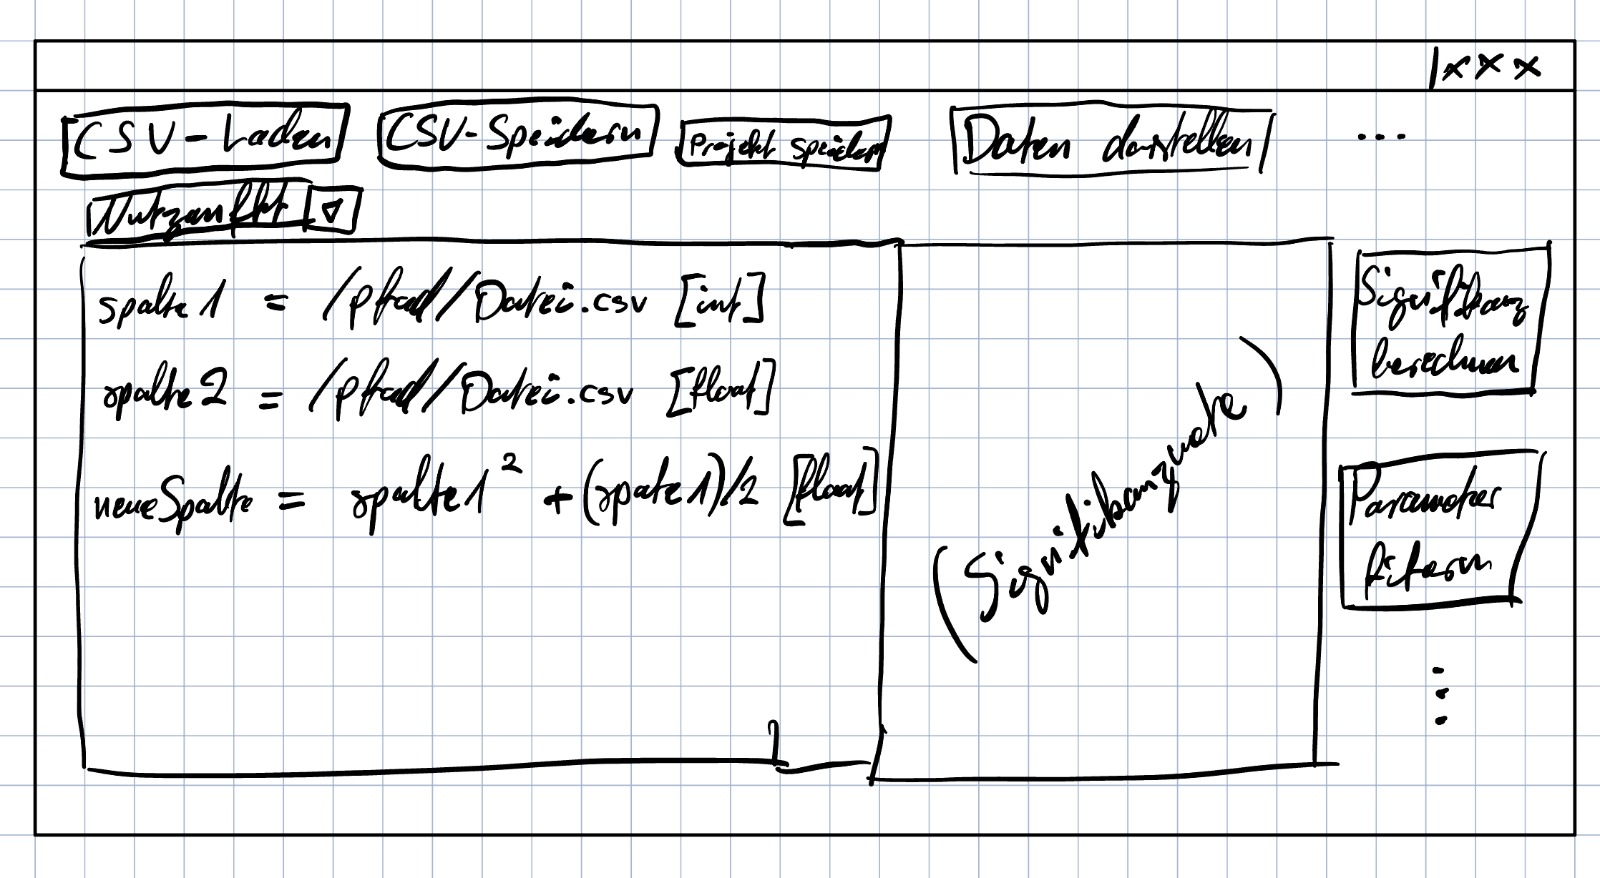
\includegraphics[width=12cm]{gui.jpeg}
  \caption{GUI Entwurf}
\end{figure}

\clearpage
\section{Globale Testfälle}

\subsection{Funktionssequenzen}
Folgende Funktionen sind zu überprüfen.

\begin{table}[H]
\begin{tabularx}{\textwidth}{rX}
\textbf{/T10/}         & \textbf{Laden der CSV Datei}                                                               \\
\textbf{Vorbedingung}  & Das Programm ist gestartet.                                                                \\
\textbf{Beschreibung}  & Der Nutzer wählt die csv Datei aus um sie zu laden. (F10)                                \\
\textbf{Nachbedingung} & Die csv Datei wurde geladen und die enthaltenen Werte vollständig vom Programm eingelesen.
\end{tabularx}
\end{table}

\begin{table}[H]
\begin{tabularx}{\textwidth}{rX}
\textbf{/T20/}         & \textbf{Speichern der CSV Datei} \\
\textbf{Vorbedingung}  & Die CSV Datei wurde vollständig geladen. Berechnungen wurden abgeschlossen.   \\
\textbf{Beschreibung}  & Der Nutzer speichert. (F11)                                \\
\textbf{Nachbedingung} & Es wurde eine neue CSV Datei erstellt, die die aktuellen Berechnungen enthält.
\end{tabularx}
\end{table}

\begin{table}[H]
\begin{tabularx}{\textwidth}{rX}
\textbf{/T21/}         & \textbf{Speichern der Signifikanzen}  \\
\textbf{Vorbedingung}  & Die CSV Datei wurde vollständig geladen. Berechnungen wurden abgeschlossen.   \\
\textbf{Beschreibung}  & Der Nutzer speichert. (F11)                               \\
\textbf{Nachbedingung} & Es wurde eine neue Datei erstellt, die die berechneten Signifikanzen enthält.
\end{tabularx}
\end{table}

\begin{table}[H]
\begin{tabularx}{\textwidth}{rX}
\textbf{/T22/}         & \textbf{Speichern der Parameter} \\
\textbf{Vorbedingung}  & Die CSV Datei wurde vollständig geladen. Berechnungen wurden abgeschlossen.   \\
\textbf{Beschreibung}  & Der Nutzer speichert. (F11) \\
\textbf{Nachbedingung} & Es wurde eine neue Datei erstellt, die die berechneten Parameter enthält.
\end{tabularx}
\end{table}

\begin{table}[H]
\begin{tabularx}{\textwidth}{rX}
\textbf{/T30/}         & \textbf{Laden vorheriger Eingaben} \\
\textbf{Vorbedingung}  & Die CSV Datei der Rohdaten wurde vollständig geladen.   \\
\textbf{Beschreibung}  & Der Nutzer wählt gespeicherte Eingaben aus und lädt sie. (F12) \\
\textbf{Nachbedingung} & Die Eingaben wurden geladen. Gespeicherte Funktionen sind dem Nutzer zugänglich. 
\end{tabularx}
\end{table}

\begin{table}[H]
\begin{tabularx}{\textwidth}{rX}
\textbf{/T40/}         & \textbf{Attributsableitung hinzufügen} \\
\textbf{Vorbedingung}  & Die CSV Datei der Rohdaten wurde vollständig geladen.   \\
\textbf{Beschreibung}  & Der Nutzer gibt eine syntaktisch korrekte Funktion ein und fügt sie hinzu. (F15) \\
\textbf{Nachbedingung} & Die Attributsableitung wird den existierenden Attributsableitungen hinzugefügt.\\

\textbf{/T40.1/}         & \textbf{Intervalle} \\
\textbf{Beschreibung}  & Der Nutzer gibt ein syntaktisch korrektes Intervall ein und fügt es als Ableitungsfunktion hinzu. (MK2.1) \\

\textbf{/T40.2/}         & \textbf{Gruppen} \\
\textbf{Beschreibung}  & Der Nutzer gibt ein syntaktisch korrekte Gruppe ein und fügt sie als Ableitungsfunktion hinzu. (MK2.2) \\

\textbf{/T40.3/}         & \textbf{Logische Ausdrücke} \\
\textbf{Beschreibung}  & Der Nutzer gibt einen syntaktisch korrekten logischen Ausdruck ein und fügt ihn als Ableitungsfunktion hinzu. (MK2.3) \\

\textbf{/T40.4/}         & \textbf{Vergleiche} \\
\textbf{Beschreibung}  & Der Nutzer gibt ein syntaktisch korrekten Vergleich ein und fügt ihn als Ableitungsfunktion hinzu. (MK2.4) \\
\end{tabularx}
\end{table}

\begin{table}[H]
\begin{tabularx}{\textwidth}{rX}
\textbf{/T41/}         & \textbf{Attributsableitung hinzufügen} \\
\textbf{Vorbedingung}  & Die CSV Datei der Rohdaten wurde vollständig geladen.   \\
\textbf{Beschreibung}  & Der Nutzer gibt eine syntaktisch inkorrekte Funktion ein und fügt sie hinzu. (F15) \\
\textbf{Nachbedingung} & Die Attributsableitung wird den existierenden Attributsableitungen nicht hinzugefügt. Der Nutzer erhält eine Warnmeldung, dass die Ableitung nicht hinzugefügt wurde aufgrund der inkorrekten Syntax.
\end{tabularx}
\end{table}

\begin{table}[H]
\begin{tabularx}{\textwidth}{rX}
\textbf{/T42/}         & \textbf{Attributsableitung ändern} \\
\textbf{Vorbedingung}  & Die CSV Datei der Rohdaten wurde vollständig geladen. Es existiert mindestens eine Attributsableitung.  \\
\textbf{Beschreibung}  & Der Nutzer wählt eine Attributsableitung aus, gibt eine syntaktisch korrekte Funktion ein und wendet die Änderung an. (F16) \\
\textbf{Nachbedingung} & Die ausgewählte Attributsableitung wird durch die geänderte Funktionsableitung ersetzt.
\end{tabularx}
\end{table}

\begin{table}[H]
\begin{tabularx}{\textwidth}{rX}
\textbf{/T43/}         & \textbf{Attributsableitung ändern} \\
\textbf{Vorbedingung}  & Die CSV Datei der Rohdaten wurde vollständig geladen. Es existiert mindestens eine Attributsableitung.   \\
\textbf{Beschreibung}  & Der Nutzer wählt eine Attributsableitung aus, gibt eine syntaktisch inkorrekte Funktion ein und wendet die Änderung an. (F16) \\
\textbf{Nachbedingung} & Die ausgewählte Attributsableitung wird nicht geändert. Der Nutzer erhält eine Warnmeldung, dass die Änderung nicht angewandt wurde aufgrund der inkorrekten Syntax.
\end{tabularx}
\end{table}

\begin{table}[H]
\begin{tabularx}{\textwidth}{rX}
\textbf{/T44/}         & \textbf{Attributsableitung löschen} \\
\textbf{Vorbedingung}  & Die CSV Datei der Rohdaten wurde vollständig geladen. Es existiert mindestens eine Attributsableitung.  \\
\textbf{Beschreibung}  & Der Nutzer wählt eine Attributsableitung aus und löscht diese. (F17) \\
\textbf{Nachbedingung} & Die ausgewählte Attributsableitung wird gelöscht.
\end{tabularx}
\end{table}

\begin{table}[H]
\begin{tabularx}{\textwidth}{rX}
\textbf{/T45/}         & \textbf{Attributsableitung anwenden} \\
\textbf{Vorbedingung}  & Die CSV Datei der Rohdaten wurde vollständig geladen. Es existiert mindestens eine Attributsableitung.  \\
\textbf{Beschreibung}  & Der Nutzer wählt eine Attributsableitung aus und wendet diese an. (F18) \\
\textbf{Nachbedingung} & Die ausgewählte Attributsableitung wird angewandt. Es wird mindestens eine neue Spalte in der CSV Datei erstellt. Mindestens eine davon enthält die Attributsberechnungen.
\end{tabularx}
\end{table}

\begin{table}[H]
\begin{tabularx}{\textwidth}{rX}
\textbf{/T50/}         & \textbf{Nutzenfunktion hinzufügen} \\
\textbf{Vorbedingung}  & Die CSV Datei wurde vollständig geladen.   \\
\textbf{Beschreibung}  & Der Nutzer gibt eine syntaktisch korrekte Funktion ein und fügt sie hinzu. (F20) \\
\textbf{Nachbedingung} & Die Nutzenfunktion wird den existierenden Nutzenfunktionen hinzugefügt.
\end{tabularx}
\end{table}

\begin{table}[H]
\begin{tabularx}{\textwidth}{rX}
\textbf{/T51/}         & \textbf{Nutzenfunktion hinzufügen} \\
\textbf{Vorbedingung}  & Die CSV Datei wurde vollständig geladen.   \\
\textbf{Beschreibung}  & Der Nutzer gibt eine syntaktisch inkorrekte Funktion ein und fügt sie hinzu. (F20) \\
\textbf{Nachbedingung} & Die Nutzenfunktion wird den existierenden Nutzenfunktionen nicht hinzugefügt. Der Nutzer erhält eine Warnmeldung, dass die Nutzenfunktion nicht hinzugefügt wurde aufgrund der inkorrekten Syntax.
\end{tabularx}
\end{table}

\begin{table}[H]
\begin{tabularx}{\textwidth}{rX}
\textbf{/T52/}         & \textbf{Nutzenfunktion ändern} \\
\textbf{Vorbedingung}  & Die CSV Datei wurde vollständig geladen. Es existiert mindestens eine Nutzenfunktion.  \\
\textbf{Beschreibung}  & Der Nutzer wählt eine Nutzenfunktion aus, gibt eine syntaktisch korrekte Funktion ein und wendet die Änderung an. (F21) \\
\textbf{Nachbedingung} & Die ausgewählte Nutzenfunktion wird durch die geänderte Nutzenfunktion ersetzt.
\end{tabularx}
\end{table}

\begin{table}[H]
\begin{tabularx}{\textwidth}{rX}
\textbf{/T53/}         & \textbf{Nutzenfunktion ändern} \\
\textbf{Vorbedingung}  & Die CSV Datei wurde vollständig geladen. Es existiert mindestens eine Nutzenfunktion.   \\
\textbf{Beschreibung}  & Der Nutzer wählt eine Nutzenfunktion aus, gibt eine syntaktisch inkorrekte Funktion ein und wendet die Änderung an. (F21) \\
\textbf{Nachbedingung} & Die ausgewählte Nutzenfunktion wird nicht geändert. Der Nutzer erhält eine Warnmeldung, dass die Änderung nicht angewandt wurde aufgrund der inkorrekten Syntax.
\end{tabularx}
\end{table}

\begin{table}[H]
\begin{tabularx}{\textwidth}{rX}
\textbf{/T54/}         & \textbf{Nutzenfunktion löschen} \\
\textbf{Vorbedingung}  & Die CSV Datei wurde vollständig geladen. Es existiert mindestens eine Nutzenfunktion.  \\
\textbf{Beschreibung}  & Der Nutzer wählt eine Nutzenfunktion aus und löscht diese. (F22) \\
\textbf{Nachbedingung} & Die ausgewählte Nutzenfunktion wird gelöscht.
\end{tabularx}
\end{table}

\begin{table}[H]
\begin{tabularx}{\textwidth}{rX}
\textbf{/T55/}         & \textbf{Linearkombination von Nutzenfunktionen anwenden} \\
\textbf{Vorbedingung}  & Die CSV Datei wurde vollständig geladen. Es existiert mindestens eine Nutzenfunktion.  \\
\textbf{Beschreibung}  & Der Nutzer wählt mindestens eine Nutzenfunktion aus und erstellt eine Linearkombination. (MK4.1) \\
\textbf{Nachbedingung} & Die konfigurierte Linearkombination der Nutzenfunktionen wird berechnet.
\end{tabularx}
\end{table}

\begin{table}[H]
\begin{tabularx}{\textwidth}{rX}
\textbf{/T60/}         & \textbf{Signifikanzberechnung} \\
\textbf{Vorbedingung}  & Die CSV Datei wurde vollständig geladen. Es existiert mindestens eine Nutzenfunktion. Alternativen wurden ausgewählt und ihnen wurden Nutzenfunktionen zugewiesen. \\
\textbf{Beschreibung}  &  \\
\textbf{Nachbedingung} & Die Signifikanzen wurden berechnet.
\end{tabularx}
\end{table}

\begin{table}[H]
\begin{tabularx}{\textwidth}{rX}
\textbf{/T61/}         & \textbf{Parameterberechnung} \\
\textbf{Vorbedingung}  & Die CSV Datei wurde vollständig geladen. Es existiert mindestens eine Nutzenfunktion. Alternativen wurden ausgewählt und ihnen wurden Nutzenfunktionen zugewiesen. \\
\textbf{Beschreibung}  &  \\
\textbf{Nachbedingung} & Die Parameter wurden berechnet.
\end{tabularx}
\end{table}

\begin{table}[H]
\begin{tabularx}{\textwidth}{rX}
\textbf{/T70/}         & \textbf{Visualisierung} \\
\textbf{Vorbedingung}  & Die CSV Datei wurde vollständig geladen. Die Signifikanzen und Paramter wurden berechnet. \\
\textbf{Beschreibung}  & (F30) \\
\textbf{Nachbedingung} & Parameter und Signifikanzen sind sichtbar. Nicht signifikante Werte werden visuell hervorgehoben dargestellt.
\end{tabularx}
\end{table}

\begin{table}[H]
\begin{tabularx}{\textwidth}{rX}
\textbf{/T71/}         & \textbf{Änderung der Schwellwerte} \\
\textbf{Vorbedingung}  & Die CSV Datei wurde geladen. Die Signifikanzen und Parameter wurden berechnet und sind sichtbar. Nicht signifikante Werte sind visuell hervorgehoben dargestellt.\\
\textbf{Beschreibung}  & Der Nutzer ändert den Schwellwert. (F35) \\
\textbf{Nachbedingung} & Änderung des Schwellwerts wurde übernommen. Reevaluierung welche Werte nicht signifikant sind. Hervorhebung der nicht signifikanten Werte.
\end{tabularx}
\end{table}

\begin{table}[H]
\begin{tabularx}{\textwidth}{rX}
\textbf{/T80/}         & \textbf{Alternativen hinzufügen} \\
\textbf{Vorbedingung}  & Die CSV Datei wurde geladen.\\
\textbf{Beschreibung}  & Der Nutzer wählt eine nicht ausgewählte Alternative aus und fügt diese hinzu. (MK3) \\
\textbf{Nachbedingung} & Die Alternative wird den bereits ausgewählten Alternativen zugefügt.
\end{tabularx}
\end{table}


\subsection{Datenkonsistenzen}
Folgende Datenkonsistenzen sind einzuhalten.
\begin{table}[H]
\begin{tabularx}{\textwidth}{rX}
\textbf{/T1000/}        & Rohdaten werden unverändert gespeichert. \\              \textbf{/T1001/}        & Das Einlesen einer gespeicherten CSV Datei resultiert im gleichen Programmzustand wie vor dem Speichervorgang.? \\
\end{tabularx}
\end{table}

\section{Qualitätsbestimmung}
\subsection{Funktionalität}
\begin{table}[H]
\centering
\begin{tabular}{lcccc}
\hline
\textbf{Produktqualität} & sehr gut & gut & normal & nicht relevant \\ \hline
Angemessenheit           &          &     & X      &                \\
Richtigkeit              & X        &     &        &                \\
Interoperabilität        &          & X   &        &                \\
Ordnungsmäßigkeit        &          &     &        & X              \\
Sicherheit               &          &     &        & X              \\  
\end{tabular}
\end{table}
Die Richtigkeit der Berechnungen nimmt höchsten Stellenwert an. Auch die Interoperabilität, insbesondere die Interaktion mit Biogeme zur Berechnung der Discrete Choice Modelle, ist wichtig. Weder Ordnungsmäßigkeit noch Sicherheit spielen eine Rolle in der Funktionalität.

\subsection{Zuverlässigkeit}
\begin{table}[H]
\centering
\begin{tabular}{lcccc}
\hline
\textbf{Produktqualität} & sehr gut & gut & normal & nicht relevant \\ \hline
Reife                    &          &     & X      &                \\
Fehlertoleranz           & X        &     &        &                \\
Wiederherstellbarkeit    &          & X   &        &                \\
\end{tabular}
\end{table}
Die Fehlertoleranz nimmt hohen Stellenwert ein um Einschränkungen an den Nutzer gering zu halten. Durch gesicherte Wiederherstellbarkeit der Projektabläufe ist Zuverlässigkeit des Programmes gegeben. 

\subsection{Benutzbarkeit}
\begin{table}[H]
\centering
\begin{tabular}{lcccc}
\hline
\textbf{Produktqualität} & sehr gut & gut & normal & nicht relevant \\ \hline
Verständlichkeit         &          & X   &        &                \\
Erlernbarkeit            &          & X   &        &                \\
Bedienbarkeit            & X        &     &        &                \\
\end{tabular}
\end{table}
Es wird besonders Wert gelegt auf die Benutzbarkeit des Baukastens durch eine sehr gute Bedienbarkeit. Das Programm soll einfach in der Anwendung sein durch seinen verständlichen und erlernbaren Ablauf.

\subsection{Effizienz}
\begin{table}[H]
\centering
\begin{tabular}{lcccc}
\hline
\textbf{Produktqualität} & sehr gut & gut & normal & nicht relevant \\ \hline
Zeitverhalten            &          &     & X      &                \\
Verbrauchsverhalten      &          &     & X      &               
\end{tabular}
\end{table}
Die Effizienz sowohl in der Zeit als auch im Speicherbedarf nimmt keinen hohen Stellenwert an. 

\subsection{Änderbarkeit}
\begin{table}[H]
\centering
\begin{tabular}{lcccc}
\hline
\textbf{Produktqualität} & sehr gut & gut & normal & nicht relevant \\ \hline
Analysierbarkeit         &          & X   &        &                \\
Modifizierbarkeit        & X        &     &        &                \\
Stabilität               & X        &     &        &                \\
Prüfbarkeit              & X        &     &        &                \\
\end{tabular}
\end{table}
Die Änderbarkeit des Programms ist von höchster Bedeutung. Das Programm soll modifizierbar sein, um verschiedene Bibliotheken zur Berechnung von Discrete Choice Modellen zu unterstützen, und die Einbindung von Algorithmen zur Erweiterbarkeit erlauben.


\clearpage

\glsaddall
\printglossary[%nonumberlist
]

\end{document}